% L4DC 2026 poster — 41.8" x 52.25" (portrait; USC ECE printable width on 42" roll)
% Build: pdflatex l4dc_poster.tex  (or latexmk -pdf l4dc_poster.tex)
% Submit: PDF attachment; request print at document size (no scaling). Subject must include
%   "poster". Target final trimmed size: 41.8" x 52.5" (height includes ~0.25" printer margin).
% Colors: USC cardinal/gold defined in RGB; ECE printer uses CMYK — export CMYK if your tool
%   allows it, otherwise expect RGB-to-CMYK conversion at print time.
\documentclass[
  25pt,
  portrait,
  margin=0mm,
  innermargin=-30mm,
  blockverticalspace=12mm,
  colspace=22mm,
]{tikzposter}

\usepackage{amsmath,amssymb}
\usepackage{graphicx}
\usepackage{booktabs}
\usetikzlibrary{shapes.geometric, arrows.meta, positioning}

% +30% font scale relative to tikzposter 25pt defaults
\renewcommand{\tiny}{\fontsize{15.6}{18.2}\selectfont}
\renewcommand{\scriptsize}{\fontsize{18.72}{23.4}\selectfont}
\renewcommand{\footnotesize}{\fontsize{22.464}{28.6}\selectfont}
\renewcommand{\small}{\fontsize{26.962}{32.5}\selectfont}
\renewcommand{\normalsize}{\fontsize{32.344}{39}\selectfont}
\renewcommand{\large}{\fontsize{38.818}{48.1}\selectfont}
\renewcommand{\Large}{\fontsize{46.579}{58.5}\selectfont}
\renewcommand{\LARGE}{\fontsize{55.9}{70.2}\selectfont}
\renewcommand{\huge}{\fontsize{67.08}{83.2}\selectfont}
\renewcommand{\Huge}{\fontsize{80.496}{100.1}\selectfont}
\DeclareMathSizes{32.344}{32.344}{26.962}{18.72}
\DeclareMathSizes{38.818}{38.818}{26.962}{18.72}
\DeclareMathSizes{46.579}{46.579}{32.344}{22.464}
\DeclareMathSizes{55.9}{55.9}{46.579}{32.344}
\DeclareMathSizes{67.08}{67.08}{46.579}{32.344}
\DeclareMathSizes{80.496}{80.496}{55.9}{38.818}

% 41.8" printable width on 42" roll; 52.25" height (0.25" short for vertical printer trim)
\geometry{paperwidth=41.8in,paperheight=52.25in}

\tikzposterlatexaffectionproofoff

% USC branding (cardinal + gold on default tikzposter style)
\definecolor{USCCardinal}{RGB}{153,0,0}
\definecolor{USCGold}{RGB}{255,204,0}
\definecolor{USCDark}{RGB}{51,51,51}

\usecolorstyle{Default}
\colorlet{titlebgcolor}{USCCardinal}
\colorlet{titlefgcolor}{white}
\colorlet{blocktitlebgcolor}{USCCardinal}
\colorlet{blocktitlefgcolor}{white}
\colorlet{blockbodybgcolor}{white}
\colorlet{blockbodyfgcolor}{USCDark}
\colorlet{innerblocktitlefgcolor}{USCCardinal}
\colorlet{notebgcolor}{USCGold!25}
\colorlet{backgroundcolor}{white}

% Full printable-width title banner (ECE attestation visible in header)
\usetitlestyle[width=\paperwidth,roundedcorners=0,linewidth=0pt,innersep=1.5cm]{Default}
\useblockstyle{Default}

% Optional logos (drop files into images/ and uncomment)
% \titlegraphic{\includegraphics[height=5.5cm]{images/usc-logo.pdf}}

\title{Online Dynamic Resource Allocation with State Constraints}
\author{Kamiar Asgari \quad Michael J. Neely}
\institute{%
  {\Large\textbf{Ming Hsieh Department of Electrical and Computer Engineering}}\\[0.35em]
  University of Southern California \quad|\quad
  8th Annual Learning for Dynamics \& Control (L4DC 2026) \quad|\quad June 17--19, 2026}

\begin{document}
\maketitle

\begin{columns}
  \column{0.5}

  \block{Motivation}{
    Many dynamic resource systems are governed by a budget state that constrains allocation at every round. The controller must act before observing inflow and cost, creating an online problem with state coupling.

    \vspace{0.4em}
    \textbf{Goal:} remain feasible at every round and compete with the best fixed policy in a tractable comparator class.

    \vspace{0.4em}
    \textbf{Applications:} energy harvesting, queueing, inventory, capital allocation, reservoir control.
  }

  \block{Problem Setup}{
    State $b_t \geq 0$, action $u_t$ with $0 \leq u_t \leq b_t$. Inflows $a_t$ and convex costs $c_t(b,u)$ may be adversarial; $u_t$ is chosen before they are revealed.

    \vspace{0.45em}
    \begin{center}
    \scalebox{1.3}{%
    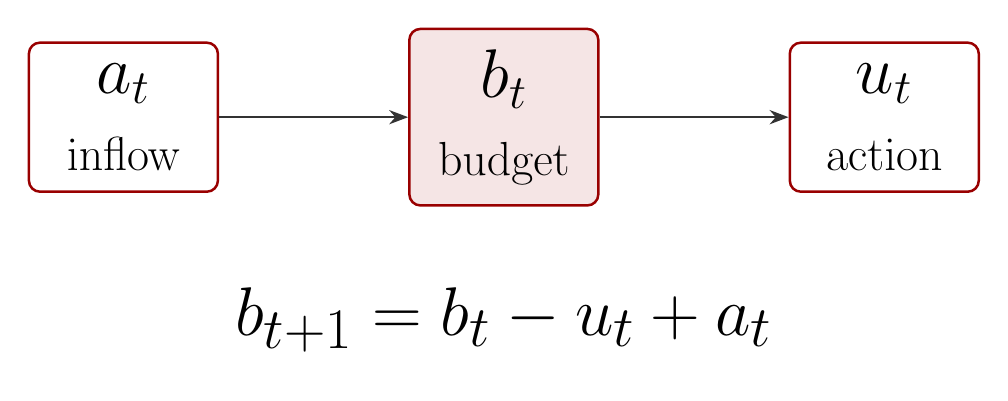
\begin{tikzpicture}[
      font=\small,
      node/.style={draw=USCCardinal, rounded corners=4pt, line width=0.9pt,
                   minimum width=2.4cm, minimum height=1.7cm, align=center},
      flow/.style={-{Stealth[length=2.4mm]}, line width=0.9pt, USCDark},
    ]
      \node[node] (inflow) {$a_t$\\[-0.2em]{\scriptsize inflow}};
      \node[node, fill=USCCardinal!10, right=2.4cm of inflow] (state)
        {$b_t$\\[-0.2em]{\scriptsize budget}};
      \node[node, right=2.4cm of state] (action)
        {$u_t$\\[-0.2em]{\scriptsize action}};

      \draw[flow] (inflow) -- (state);
      \draw[flow] (state) -- (action);

      \node[below=0.75cm of state, font=\normalsize] {$b_{t+1} = b_t - u_t + a_t$};
    \end{tikzpicture}}
    \end{center}

    \vspace{0.35em}
    \textbf{Objective:} low cumulative cost vs.\ the best fixed comparator policy in hindsight, with feasibility throughout.
  }

  \block{Key Contributions}{
    \begin{itemize}
      \item \textbf{SDAC policy class} --- simplex-constrained disturbance-action policies that preserve feasibility by construction.
      \item \textbf{Online controller} over SDAC weights with sublinear horizon and logarithmic policy-dimension regret.
      \item \textbf{Adversarial setting} --- general convex state--action costs without distributional assumptions.
    \end{itemize}
  }

  \block{Simplex Disturbance-Action Control (SDAC)}{
    % TODO: add SDAC figure from manuscript
    \centering
    \fbox{\parbox[c][7cm][c]{0.92\linewidth}{\centering\Large\textit{[SDAC policy diagram / equations]}}}
  }

  \column{0.5}

  \block{Online Algorithm}{
    \textbf{Inputs:} horizon $T$, step size $\eta>0$, gain $\kappa\in(0,1]$, memory $H$, initial weights $w_1\in\Delta_H$, $b_1=0$.

    \vspace{0.35em}
    \textbf{Each round $t=1,\ldots,T$} (choose action \emph{before} seeing $a_t,c_t$):

    \begin{enumerate}
      \item \textbf{Propose} an SDAC action from current weights:
        \[
          \widehat{u}_t \leftarrow \kappa b_t + \langle w_t,\widetilde{a}_t\rangle,
          \qquad
          \widetilde{a}_t^{(i)}=(1-\kappa)^i a_{t-i}.
        \]
      \item \textbf{Clip} to the available budget (feasibility):
        \[
          u_t \leftarrow \min\{\widehat{u}_t,\, b_t\}.
        \]
      \item \textbf{Update state} after inflow $a_t$ arrives:
        \[
          b_{t+1} \leftarrow b_t - u_t + a_t.
        \]
      \item \textbf{Learn} from the revealed cost $c_t(b_t,u_t)$: build a convex surrogate
        $\ell_t(w)=c_t\bigl(b_t^{\pi(w)},u_t^{\pi(w)}\bigr)$ and take one exponentiated-gradient step on the simplex,
        \[
          w_{t+1}^{(i)} \propto w_t^{(i)}\exp\!\bigl(-\eta\, g_t^{(i)}\bigr),
          \qquad g_t\in\partial\ell_t(w_t),
        \]
        then renormalize so $w_{t+1}\in\Delta_H$.
    \end{enumerate}
  }

  \block{Regret Guarantee}{
    % TODO: main theorem statement
    \fbox{\parbox[c][5.5cm][c]{0.92\linewidth}{\centering\Large\textit{[Main regret bound]}}}
  }

  \block{Experiments}{
    % TODO: result plots
    \fbox{\parbox[c][7cm][c]{0.92\linewidth}{\centering\Large\textit{[Experimental results]}}}
  }

  \block{Takeaways}{
    SDAC encodes feasibility structurally, enabling clean adversarial regret analysis for state-coupled resource allocation.

    \vspace{0.4em}
    \textbf{Contact:} \texttt{kamiar@usc.edu}
  }

\end{columns}

\node[anchor=south,font=\normalsize,text=USCDark!70]
  at (bottomleft) {Poster size: 41.8\,$''$ $\times$ 52.25\,$''$ document (42\,$''$ roll; $\sim$52.5\,$''$ after vertical trim)};

\end{document}
